% "Станет проще"

\documentclass[a4paper,12pt]{article} % тип документа

% report, book

% Рисунки
\usepackage{graphicx}
\usepackage{wrapfig}
\usepackage{hyperref}
\usepackage[rgb]{xcolor}
\pagestyle{plain}



%  Русский язык

\usepackage[T2A]{fontenc}			% кодировка
\usepackage[utf8]{inputenc}			% кодировка исходного текста
\usepackage[english,russian]{babel}	% локализация и переносы
\usepackage[normalem]{ulem} 

% Математика
\usepackage{amsmath,amsfonts,amssymb,amsthm,mathtools} 


\usepackage{wasysym}

%Заговолок
\author{Сафиуллин Роберт	}
\title{Лабораторная работа 3.5.3\\ Релаксационные колебания}





\begin{document} % начало документа

\maketitle


\newpage
\section{Цель работы:}
 изучение вольт-ампернйо характеристики нормального тлеющего разряда; исследование релаксационного генератора на стабилитроне.
\\
стабилитрон СГ-2, амперметр, вольтметр, магазин сопротивлений, магазин емкостей, источник питания, осциллограф, генератор звуковой частоты
 
\section{Экспериментальная установка:}
\begin{center}
\includegraphics[scale=0.3]{ust1}
\includegraphics[scale=0.5]{ust2}

\end{center}

\section{Ход работы}

\textbf{I: Характеристика стабилитрона}\\
1) Собрали первую схему\\
2) Сняли вольт-амперную характеристику. Также посчитали напряжение для стабилитрона без сопротивления r=5.1 $k\Omega$, вычитая падение напряжения на r при каждом токе. Результаты занессли в таблицу: \\
\begin{tabular}{|c|c|c|c|c|c|c|}
\hline 
V, В & $V_{\sout{r}}$ & I, *0.25 mA & $V_z$, В & $I_z$, *0.25 mA & $V_g$, В & $I_g$, *0.25 mA     \\ 
\hline 
87 &  73& 11 & 96.9 & 18 & 75 & 2.3   \\ 
\hline 
84.7 & 71.95 & 10 & 97 & 18.5 & 75.7 & 2.2   \\ 
\hline 
82 & 71.8 &8 & 97.03 & 19.3 &  &    \\ 
\hline 
81.4 & 72.5 & 7 &  &  &  &    \\ 
\hline 
79.7 &  72& 6 &  &  &  &    \\ 
\hline 
78.2 & 71.8 & 5 &  &  &  &    \\ 
\hline 
77.2 & 72.1 & 4 &  &  &  &     \\ 
\hline 
75.9 & 72.7 & 2.5 &  &  &   &    \\ 
\hline 
97 & 79.15 & 14 &  &  &  &   \\ 
\hline 
93 & 73.9& 15 &  &  &  &     \\ 
\hline 
94 &  73.6& 16 &  &  &  &     \\ 
\hline 
89 & 73.7& 12 &  &  &  &     \\ 
\hline 
85 & 71.95  &10 &  &  &  &     \\ 
\hline 
84 & 72.5 & 9 &  &  &  &     \\ 
\hline 
\end{tabular} 

Построим графики напряжения с и без сопроивления:\\
\begin{center}

\includegraphics[scale=0.4]{3531} \\
\end{center}

3) Собрали релаксационный генератор(вторую схему) и получили картинку пилообразных колебаний: \\
\begin{center}

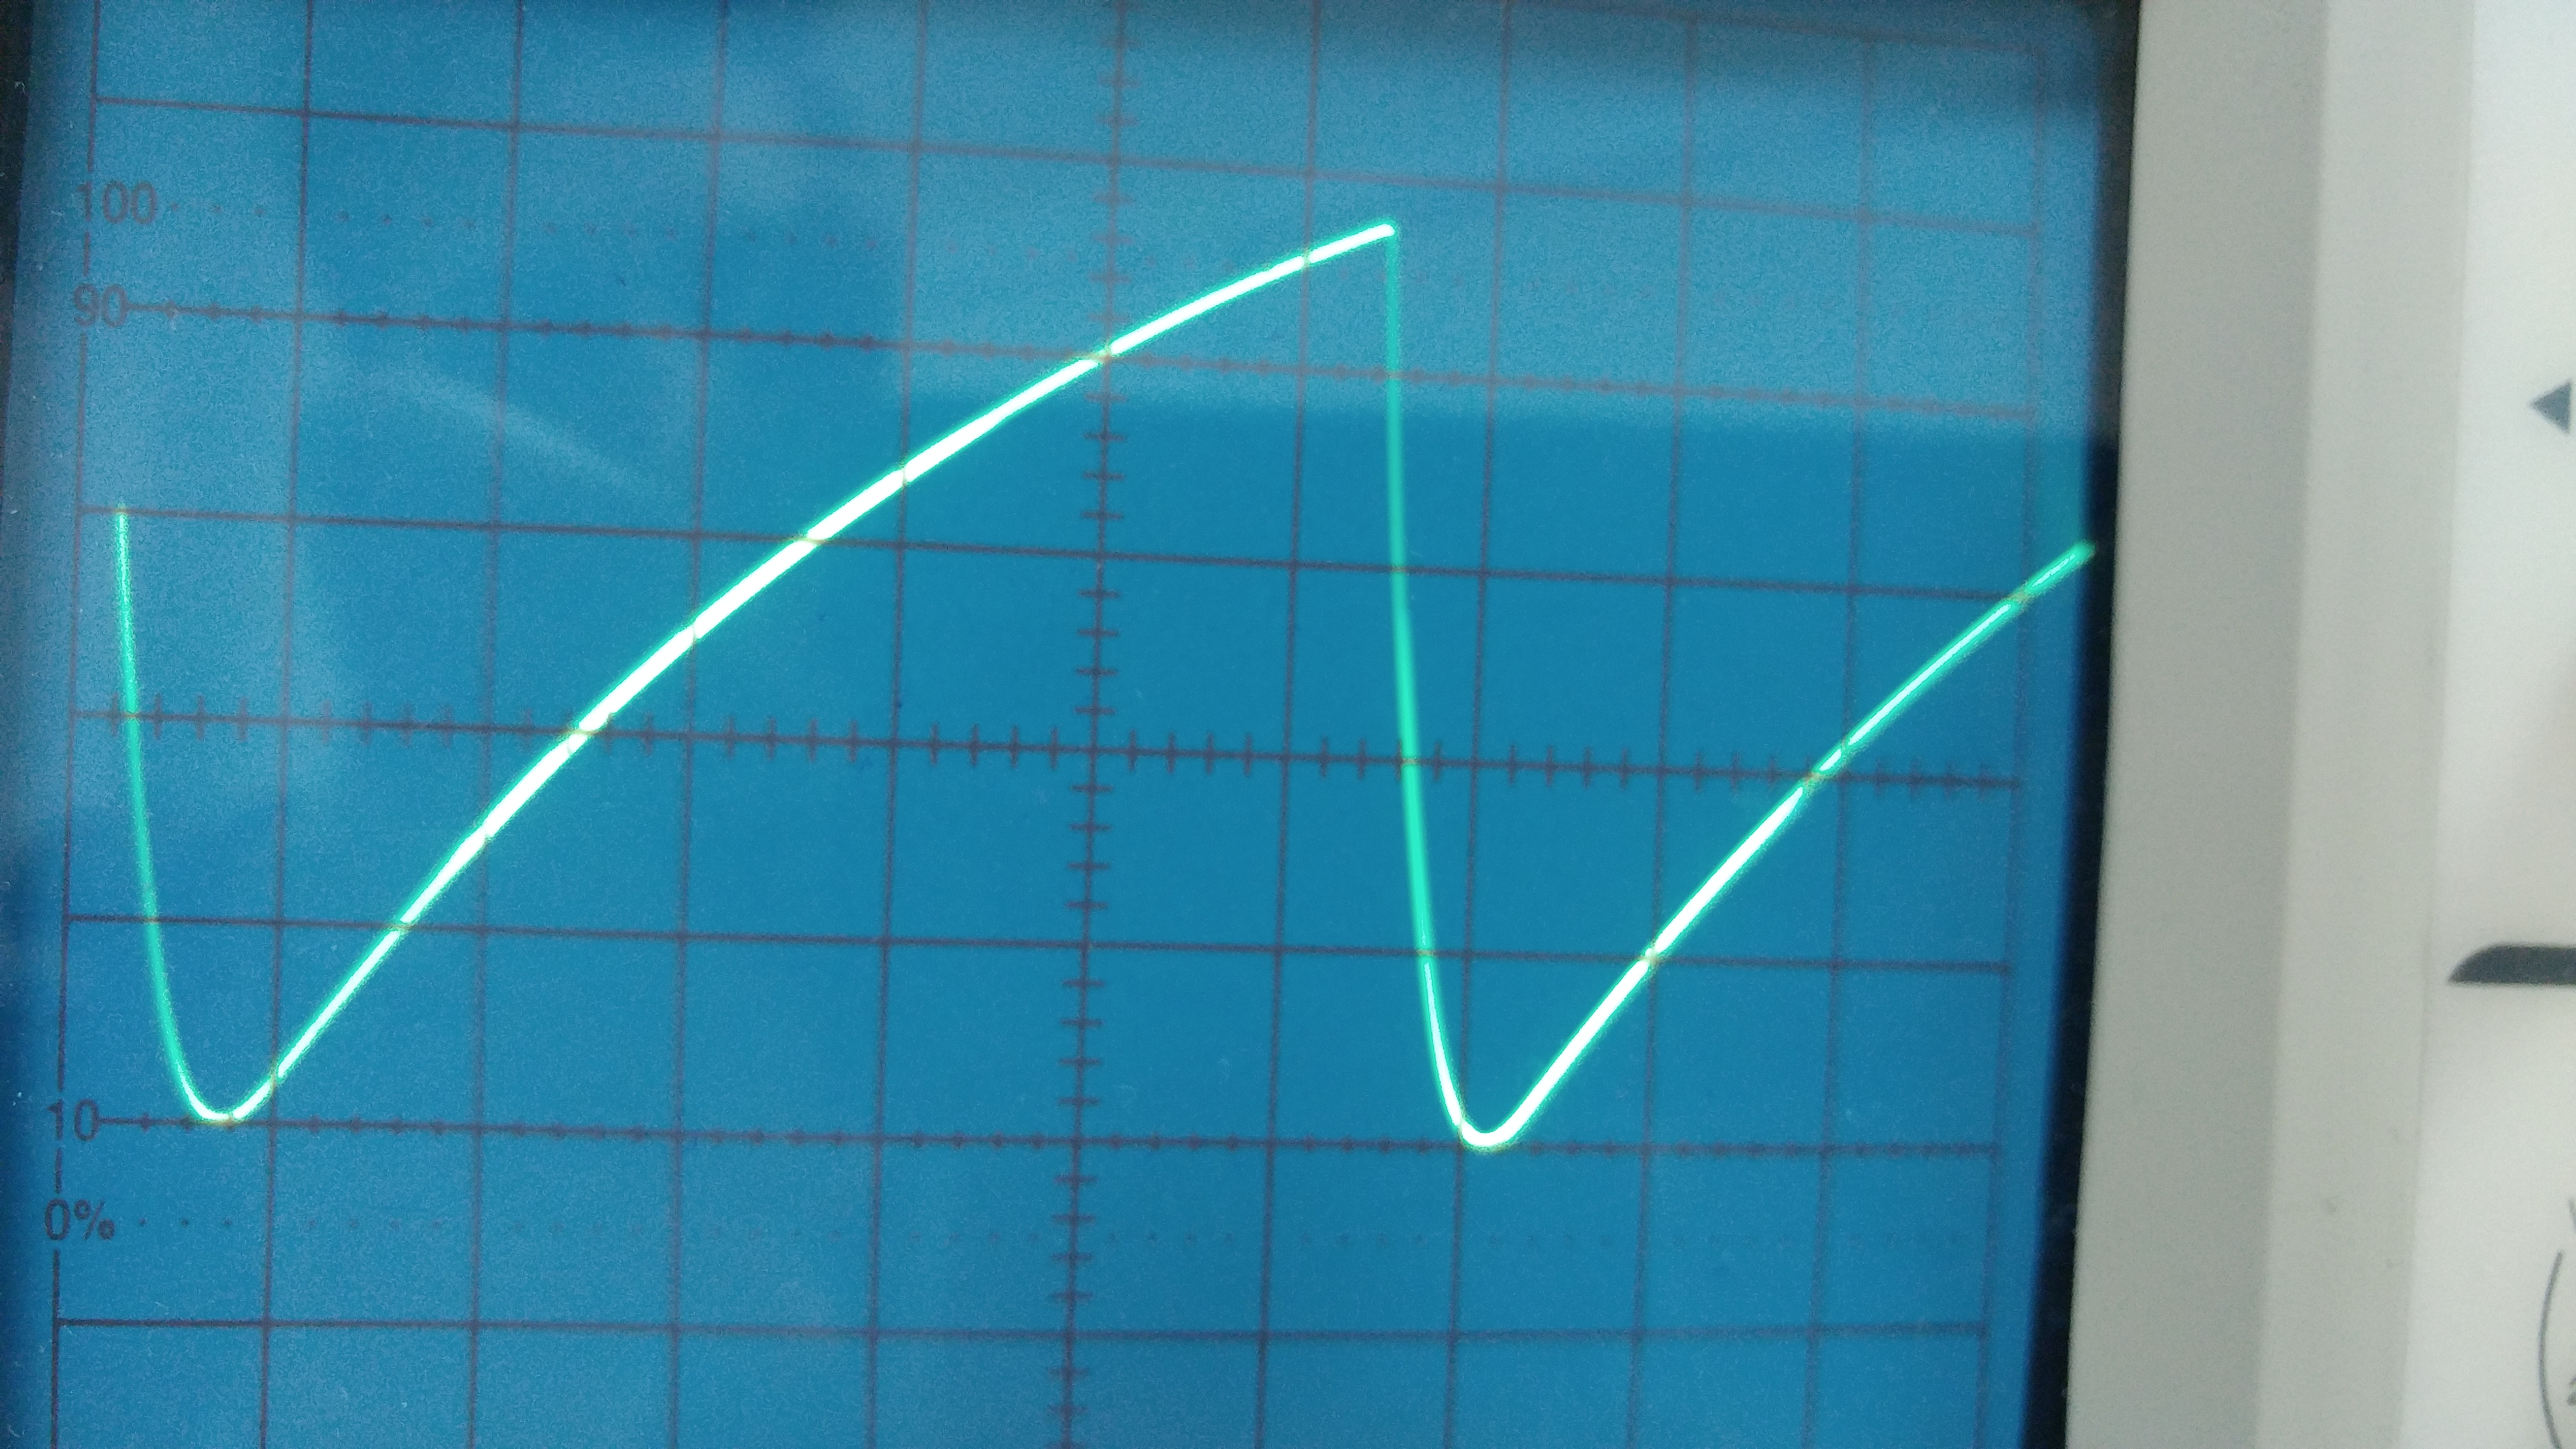
\includegraphics[scale=0.031]{kol}\\
\end{center}

4) Оценим время зарядки и разрядки: $\tau_z=11.2 mS, \tau_r=1 mS$\\
5) Также установили критическое сопротивление, при котором пропадают колебания: $R_{kr}=135 k\Omega$, теоретическое значение: $R_{kr}^{teor}=\frac{U-V_g}{I_g}=86k\Omega$\\



6) Установим параметры: $ C=5*10^{-2}  mkF, R=900 k\Omega,  U\sim1.2V_z $\\
7) Подберем подходящую частоту и получим фигуру Лиссажу без самопересечений для отношения частот :

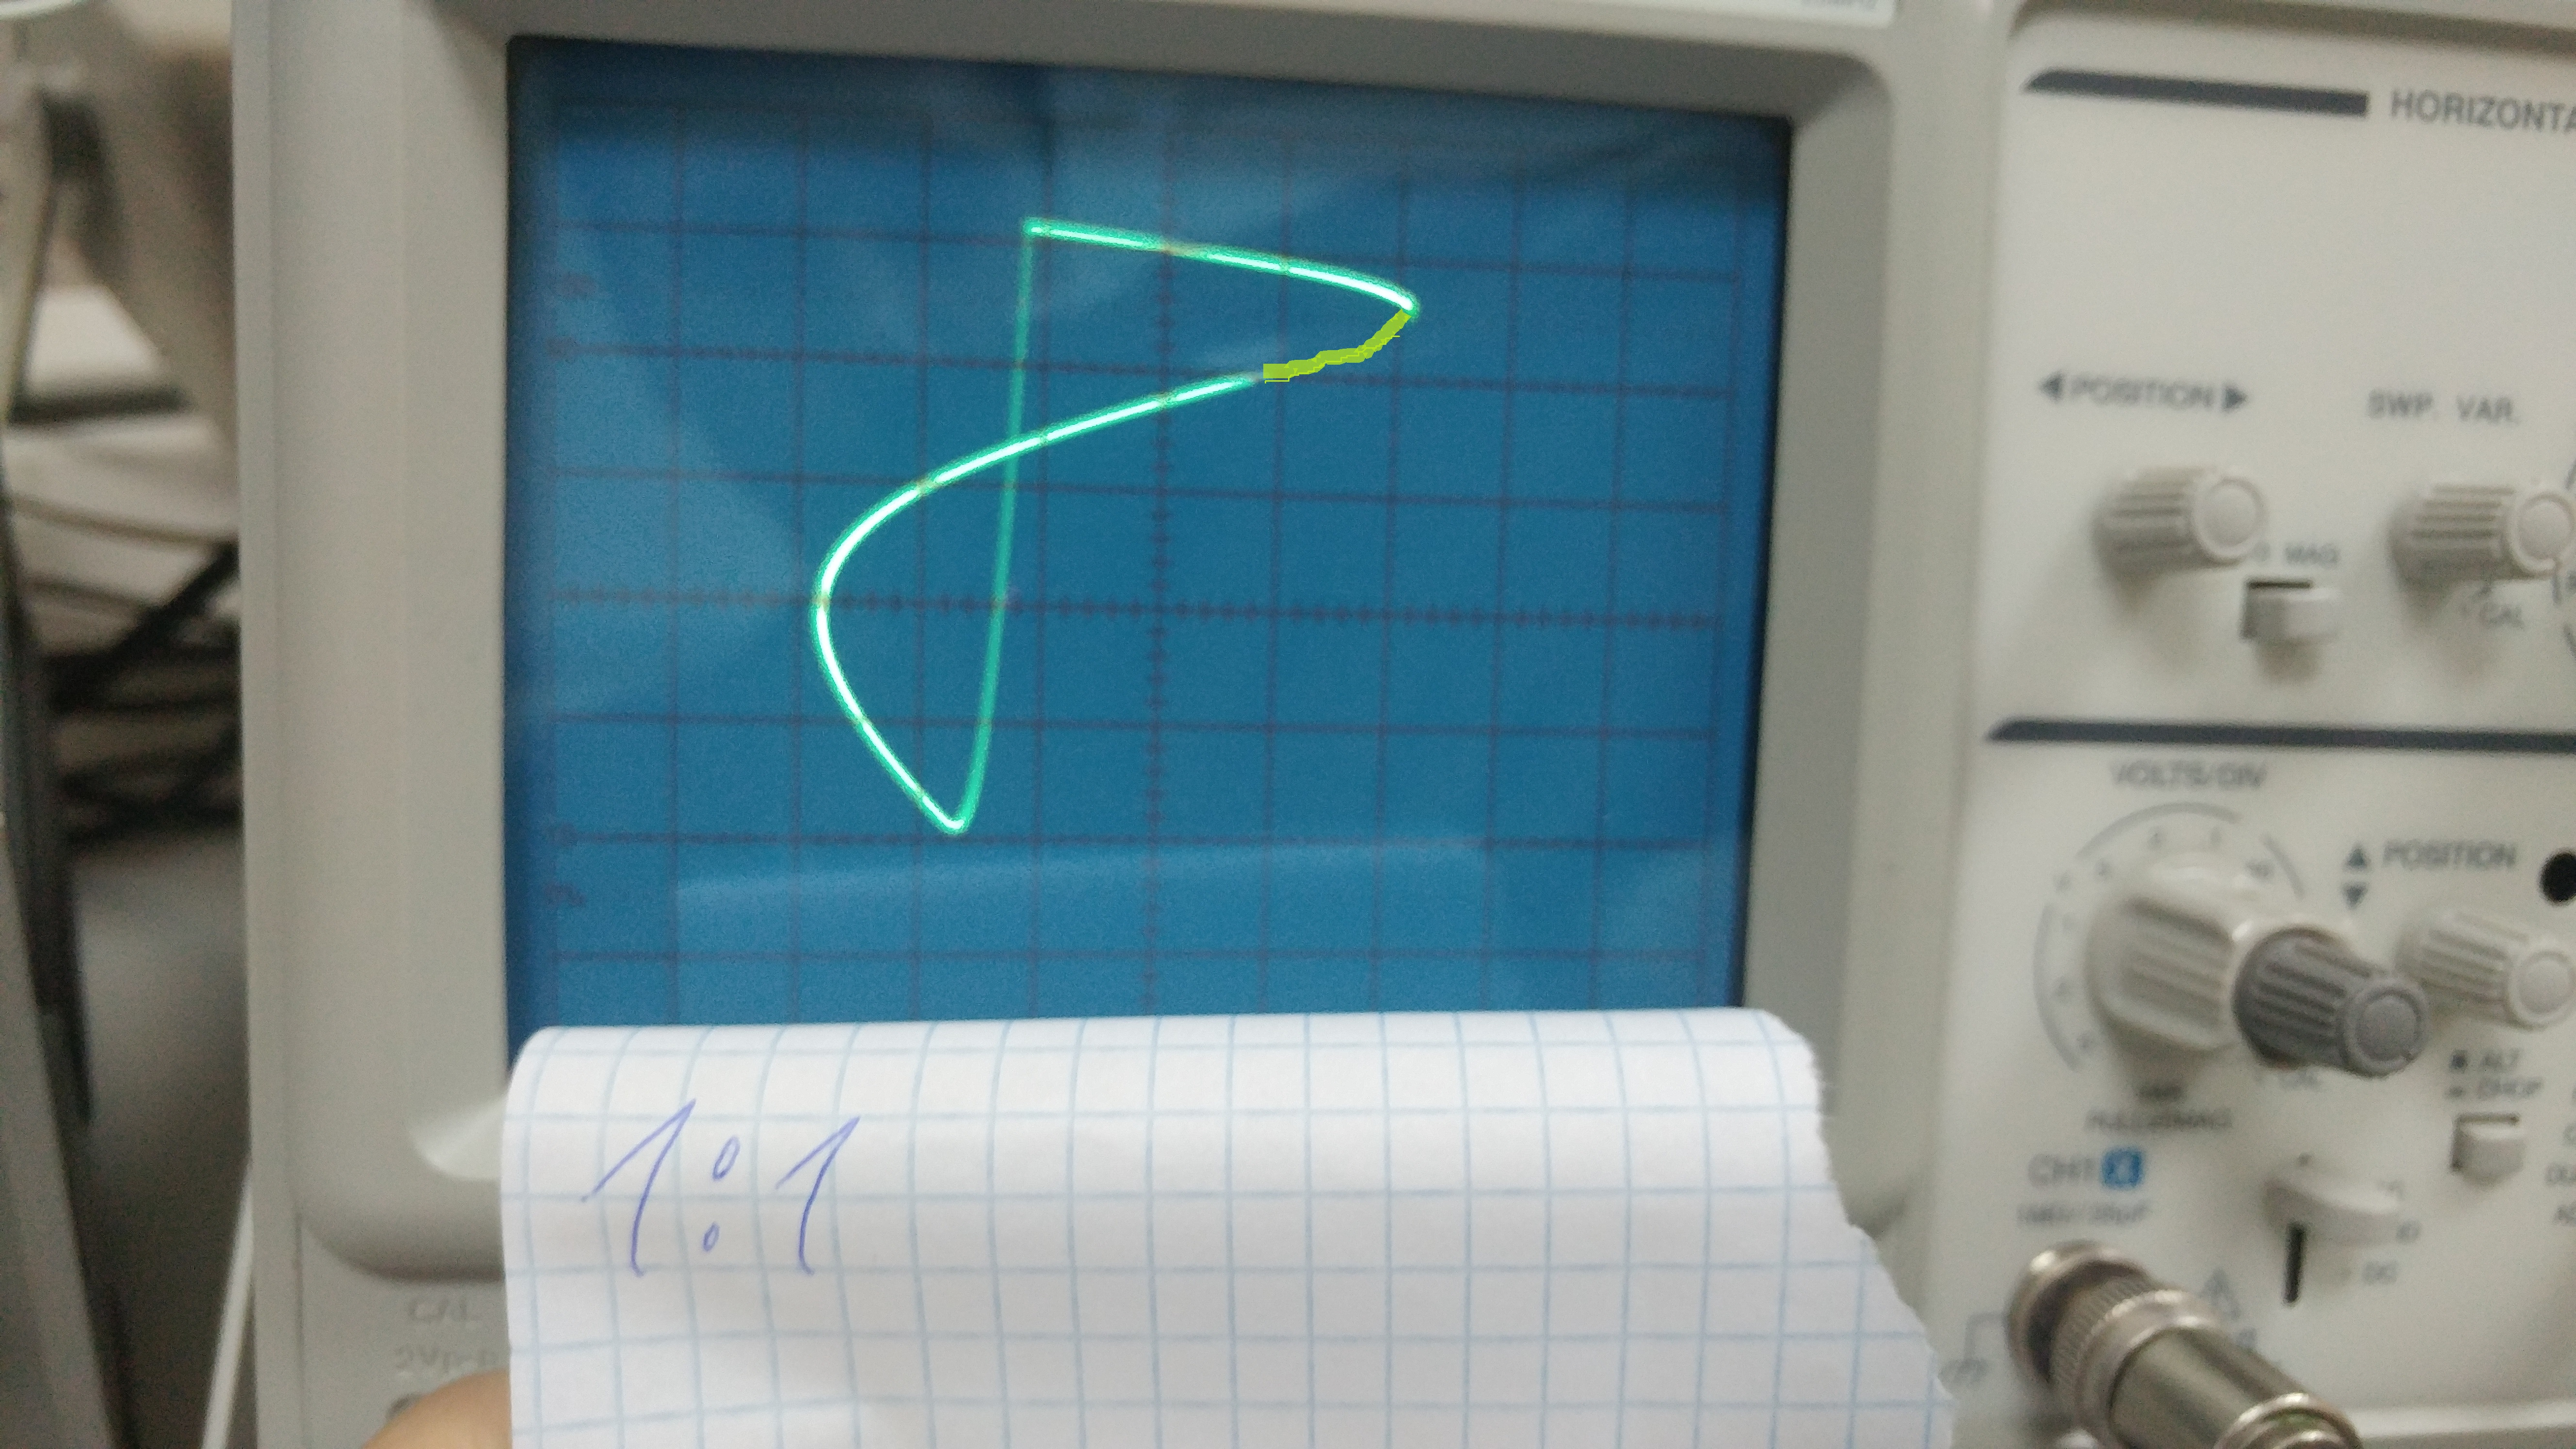
\includegraphics[scale=0.05]{11}
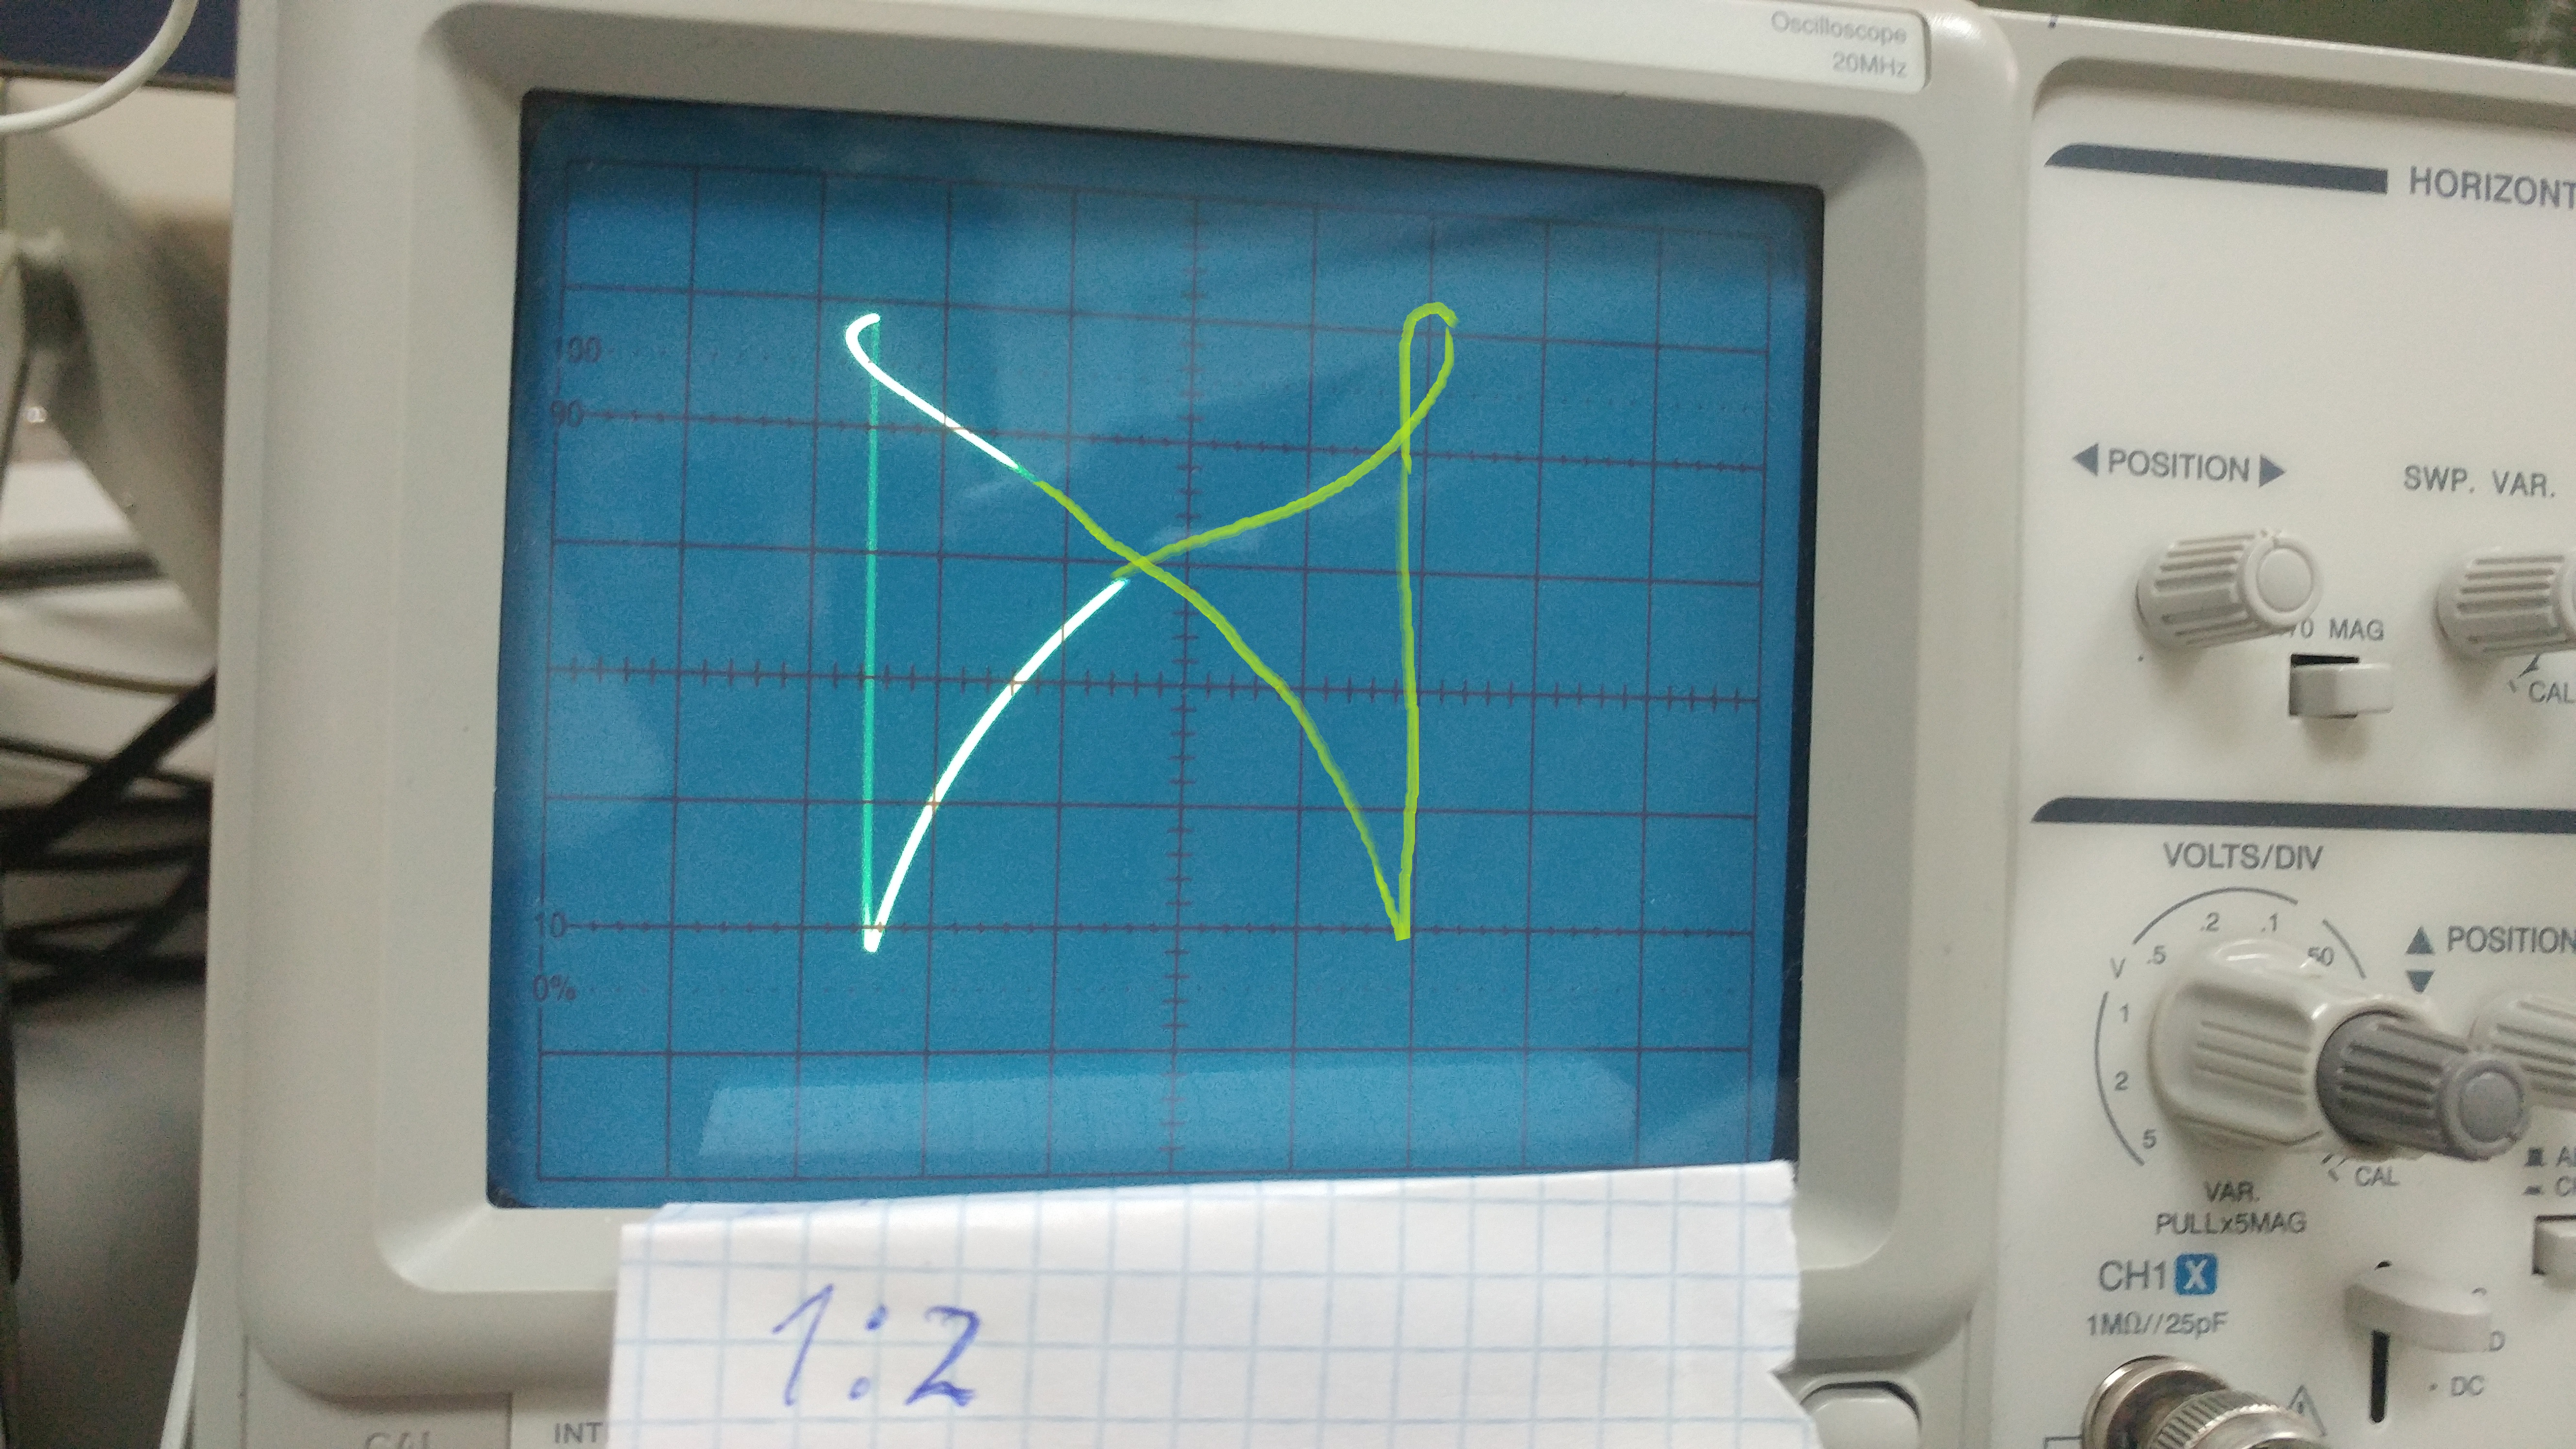
\includegraphics[scale=0.05]{12}
\includegraphics[scale=0.05]{13}
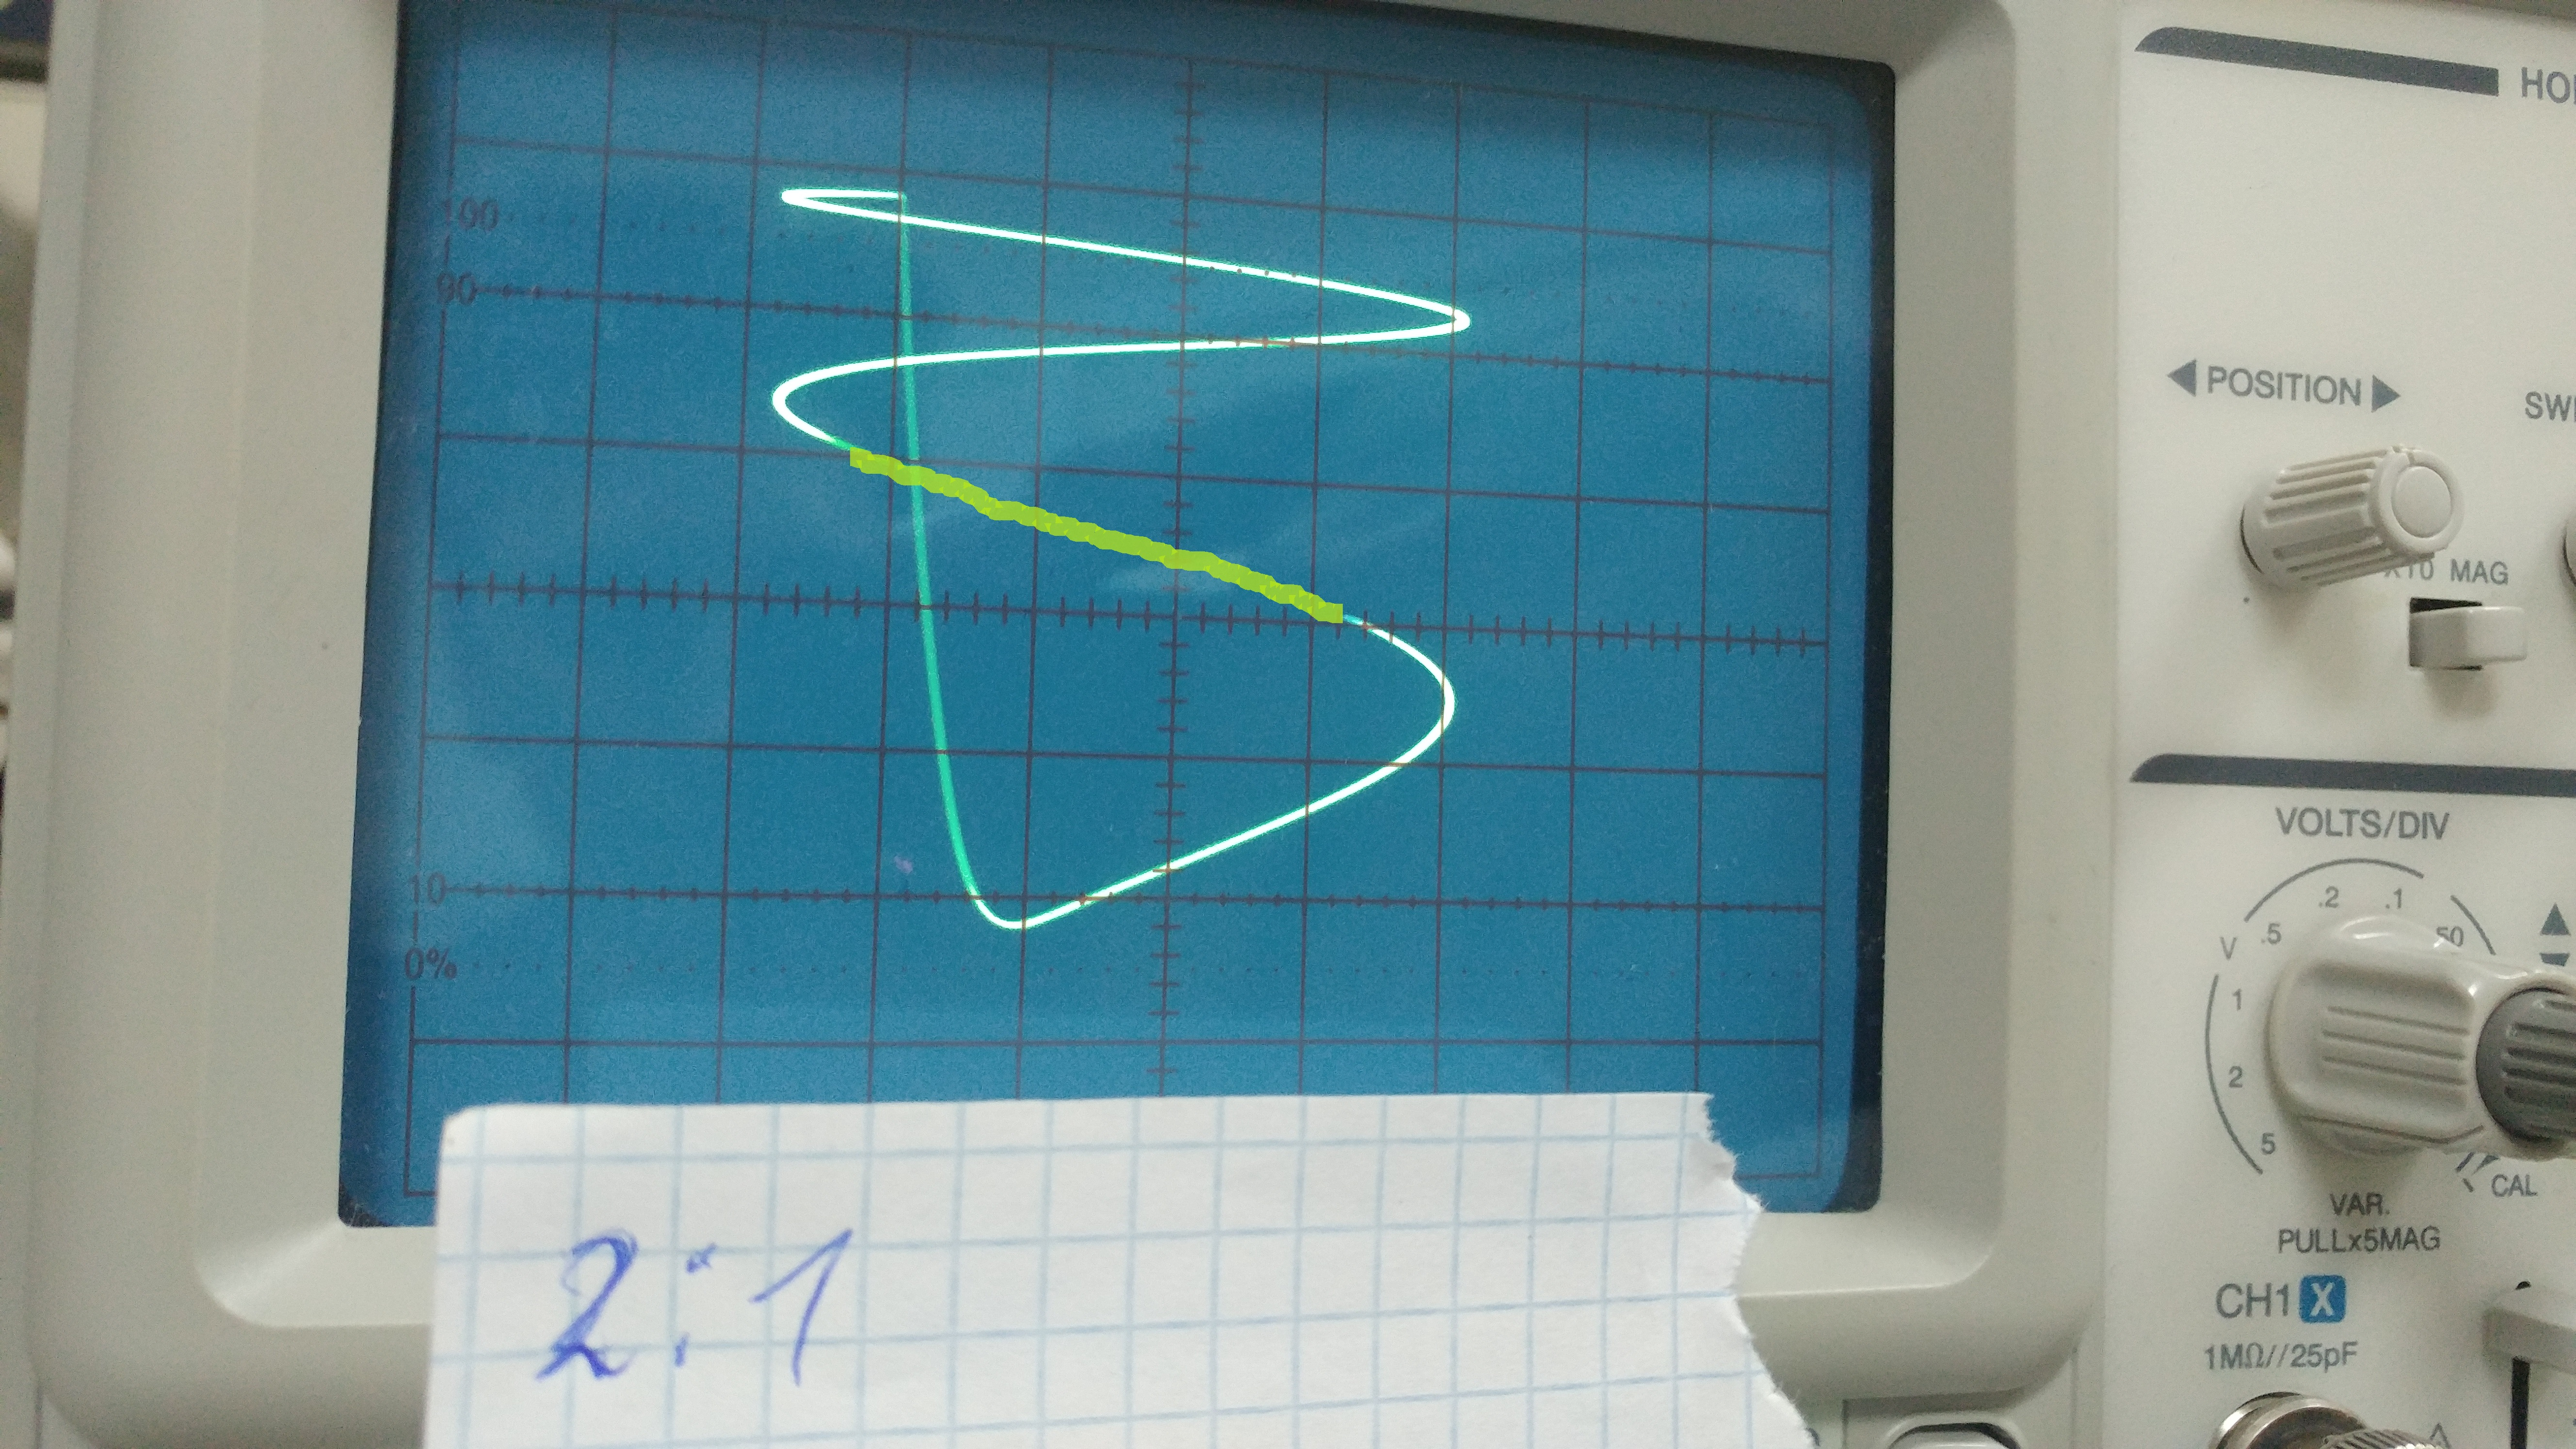
\includegraphics[scale=0.05]{21}
\begin{center}

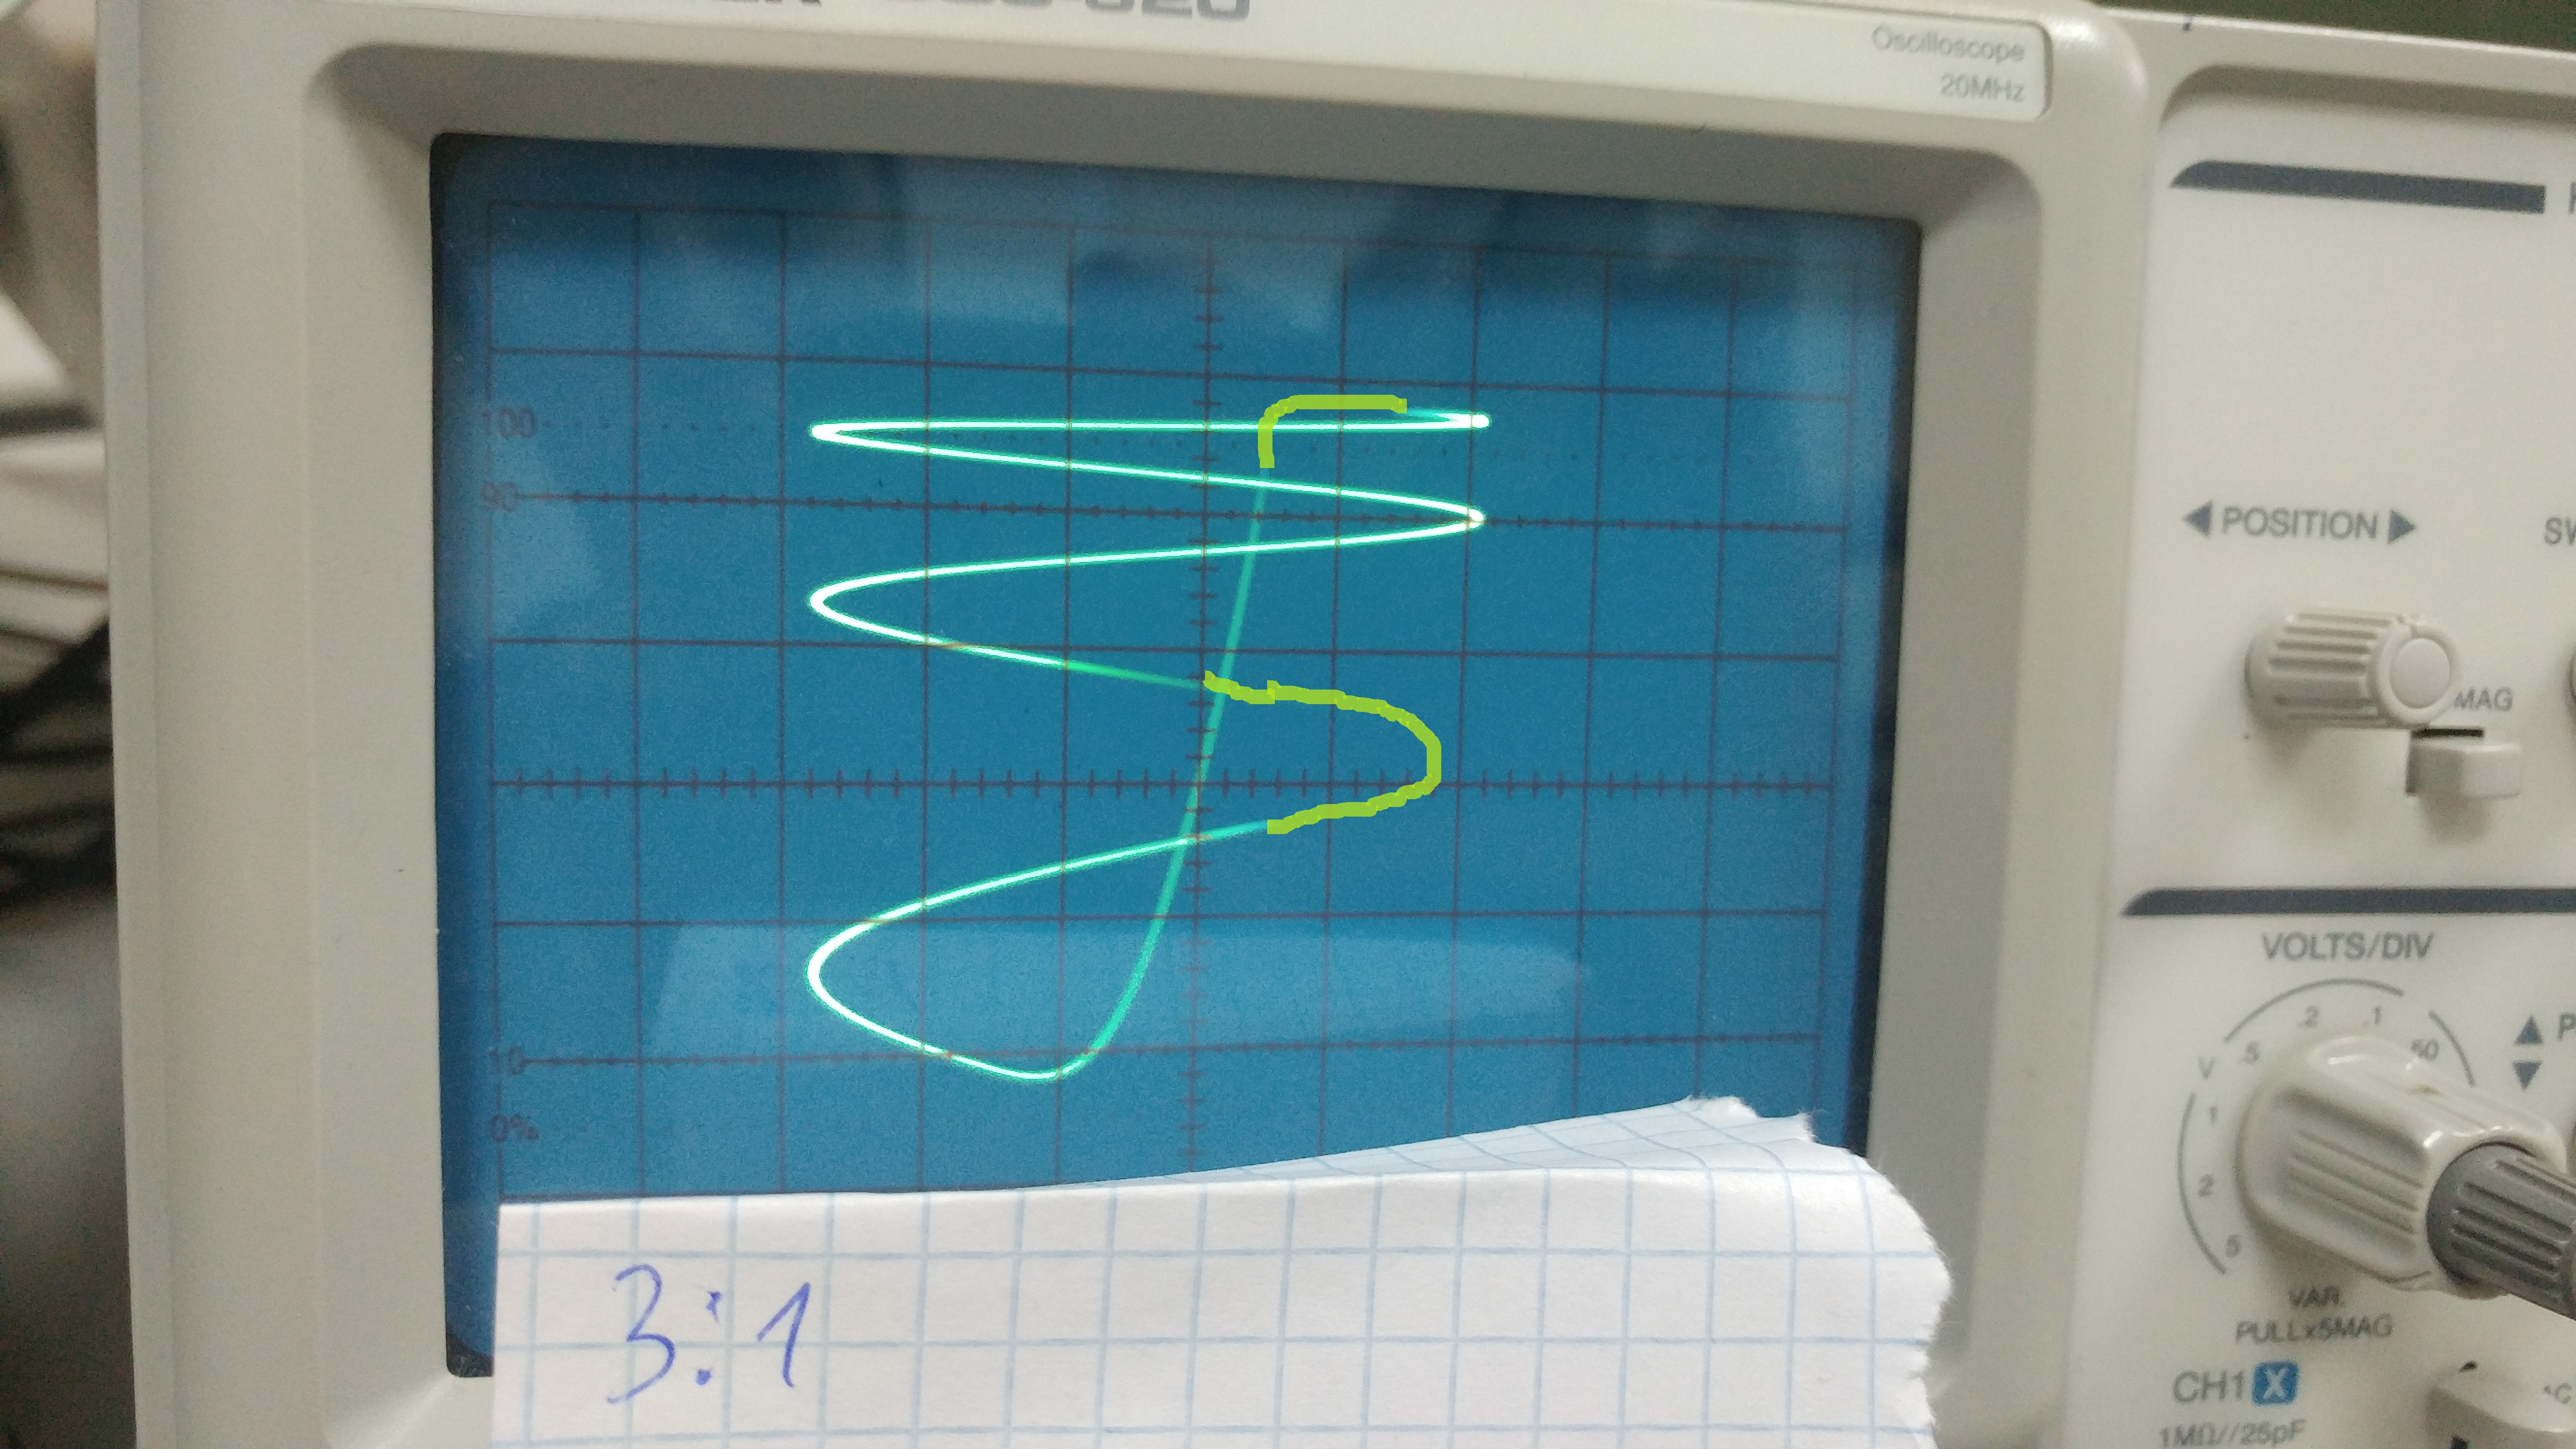
\includegraphics[scale=0.04]{31}

\end{center}



8) Установим напряжение, равное $3R_{kr}$ и снимем с помощью фигур Лиссажу зависимость частоты колебаний от емкости. Также рассчитаеем экспериментальное и теоретическое значения периода, используя формулу: $T=RC\ln\frac{U-V_2}{U-V1}$\\ Результаты занесем в таблицу:\\
\begin{tabular}{|c|c|c|c|}
\hline 
C, $10^{-2}  mkF$	 & $\nu$, Гц & $T_{exp}$, mS & $T_{teor}$, mS \\ 
\hline 
5 & 61.1 & 16.4 & 2.8 \\ 
\hline 
4 & 77.2 & 13 & 2.2 \\ 
\hline 
3 & 105 & 9.5 & 1.7 \\ 
\hline 
2 & 171 & 5.9 & 1.1 \\ 
\hline 
1 & 401 & 2.5 & 0.6 \\ 
\hline 
0.9 & 409 & 2.5 & 0.5 \\ 
\hline 
0.8 & 509 & 2 & 0.4 \\ 
\hline 
0.5 & 1070 & 0.9 & 0.3 \\ 
\hline 
\end{tabular} 



Построим по ней график:\\
\begin{center}
\includegraphics[scale=0.3]{3532}
\end{center}


9) Проведем измерения частоты при переменном сопротивлении и постоянной емкости C=$5*10^{-2}  mkF$. Результаты, вместе с теоретическими, также запишем в таблицу: \\
\begin{tabular}{|c|c|c|c|}
\hline 
R, $k\Omega$ & $\nu$, Гц  & $T_{exp}$, mS & $T_{teor}$, mS \\ 
\hline 
990 & 22 & 45.5 & 31.7 \\ 
\hline 
890 & 26 & 38.5 & 28.5 \\ 
\hline 
790 & 30 & 33.3 & 25.3 \\ 
\hline 
690 & 34 & 29.4 & 22.1 \\ 
\hline 
590 & 39.5 & 25.3 & 18.9 \\ 
\hline 
490 & 47.7 & 21 & 15.7 \\ 
\hline 
390 & 60 & 16.7 & 12.5 \\ 
\hline 
290 & 81.6 & 12.3 & 9.3 \\ 
\hline 
180 & 134 & 7.5 & 5.8 \\ 
\hline 
170 & 146 & 6.9 & 5.4 \\ 
\hline 
160 & 157 & 6.4 & 5.1 \\ 
\hline 
150 & 176 & 5.7 & 4.8 \\ 
\hline 
141 & 196 & 5.1 & 4.5 \\ 
\hline 
\end{tabular} 
\\
Построим график зависимости T(R): \\
\begin{center}
\includegraphics[scale=0.3]{3533}
\end{center}
















































































\end{document} % конец документа
